%%%%% vpc
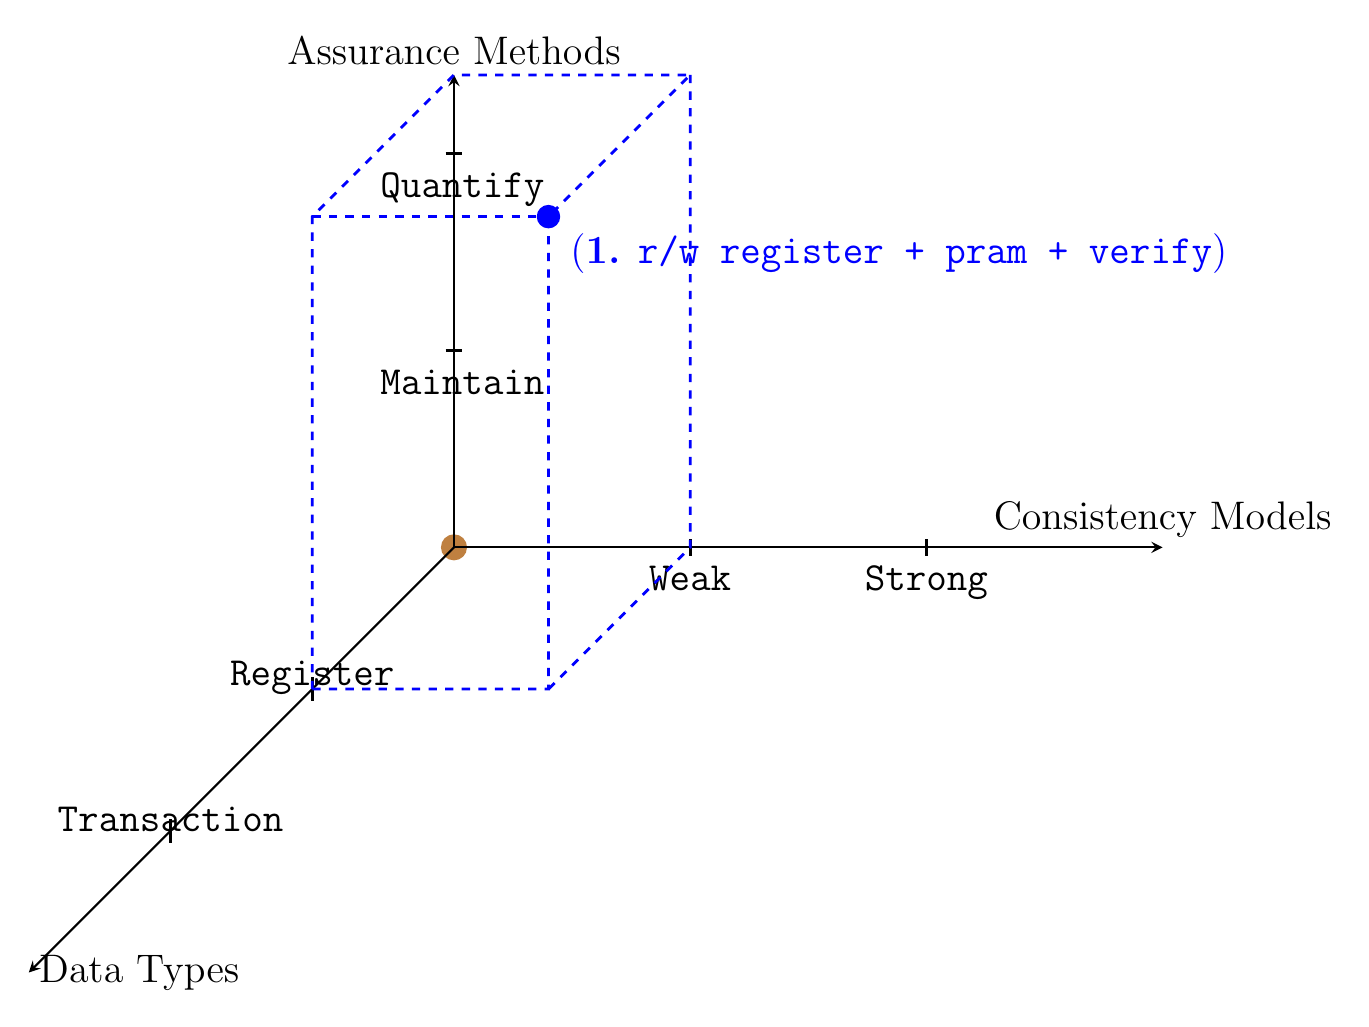
\begin{tikzpicture}[x = 0.5cm, y = 0.5cm, z = 0.3cm, >=stealth, font = \Large]

\node[fill = brown, circle] at (0,0,0) {};
% The axes
\draw[->, thick] (xyz cs:x=0) -- (xyz cs:x = 18) node[above, font = \Large] {$\textrm{Consistency Models}$};
\draw[->, thick] (xyz cs:y=0) -- (xyz cs:y = 12) node[above, font = \Large] {$\textrm{Assurance Methods}$};
\draw[->, thick] (xyz cs:z=0) -- (xyz cs:z = -18) node[right, font = \Large] {$\textrm{Data Types}$};

% The ticks

% ticks for consistency models
\draw[very thick] (6,-3pt) -- (6,3pt) node[below = 6pt, align = center] {\texttt{Weak}};
\draw[very thick] (12,-3pt) -- (12,3pt) node[below = 6pt, align = center] {\texttt{Strong}};

% ticks for assurance methods
\draw[very thick] (-3pt,5) -- (3pt,5) node[below = 3pt] {\texttt{Maintain}};
\draw[very thick] (-3pt,10) -- (3pt,10) node[below = 3pt] {\texttt{Quantify}};

% ticks for data types
\draw[very thick] (xyz cs:y=-0.3pt,z=-6) -- (xyz cs:y=0.3pt,z=-6) node[align = center] { \texttt{Register}}; 
\draw[very thick] (xyz cs:y=-0.3pt,z=-12) -- (xyz cs:y=0.3pt,z=-12) node[align = center] 
{\texttt{Transaction}}; 

% register + weak (pram) + quantify (verify)
  \begin{scope}[line width = 1, blue]
	\draw[dashed] 
	  (xyz cs:z = -6) coordinate (z) -- 
	  (xyz cs:y = 12, z = -6) coordinate (yz) --
	  (xyz cs:x = 0, y = 12, z = 0) coordinate (y) -- 
	  (xyz cs:x = 6, y = 12) coordinate (xy) --
	  (xyz cs:x = 6, y = 12, z = -6) coordinate (xyz) --
	  (xyz cs:x = 6, z = -6) coordinate (xz) -- cycle;
	\draw[dashed, line width = 1, blue] (yz) -- (xyz);
	\draw[dashed, line width = 1, blue] (xy) -- (6,0) -- (xz);
	
	% Dots and labels for P, Q
	\node[fill = blue, circle, inner sep = 3pt, label = {[blue, font = \Large] -30: (\textbf{1.} 
  \texttt{r/w register + pram + verify})}] at (xyz) {};
  \end{scope}
\end{tikzpicture}
